En este apartado se presenta el análisis del estudio de factibilidad el cual se ha estructurado en tres campos principales: Factibilidad Técnica, Factibilidad Operativa y Factibilidad Económica.  Se formula con base en información que tiene la menor incertidumbre posible para medir las posibilidades de éxito o fracaso de un proyecto de inversión, apoyándose en él se tomará la decisión de proceder o no con su implementación. 

\subsection{Factibilidad técnica}
\label{sec:factibilidad_tecnica}
%---------------------
%FACTIBILIDAD TÉCNICA
%---------------------
Para determinar la factibilidad técnica es necesario evaluar los aspectos tecnológicos del proyecto para  averiguar si es posible desarrollar el nuevo sistema teniendo en cuenta los recursos técnicos actuales\cite{kendall_analisis}. De esta manera y debido a las características propias del prototipo, se evalúa únicamente el software necesario para conseguir una plataforma para desarrollar la aplicación móvil y el sistema para almacenar la base de datos con soporte para análisis geoespacial. 

\subsubsection{Software}
\label{subsubsec: software}
Primero, para el desarrollo del prototipo móvil es necesario la utilización de un marco de trabajo que nos permita realizar aplicaciones móviles para android. Múltiples candidatos cumplen con los requisitos básicos. La tabla \ref{tab:tabla-comparativa-framework} muestra una comparativa entre las opciones nativas y frameworks multi-plataforma más populares del mercado.


\begin{table}[h]
\centering
\scriptsize
\renewcommand{\arraystretch}{1.5}
\caption{Comparación de tecnologías de desarrollo de aplicaciones móviles}
\begin{tabularx}{\textwidth}{ |C|C|C|C| }
\hline
\textbf{Característica} &
\textbf{Flutter} &
\textbf{Kotlin} &
\textbf{React Native}
\\ \hline
Lenguaje base &
Dart \cite{flutter_businessvalue} &
Kotlin \cite{kotlin_docs}&
JavaScript \cite{reactnative_docs}
\\ \hline
Renderizado de la interfaz &
Motor propio (Impeller) \cite{flutter_businessvalue} &
Componentes nativos \cite{kotlin_docs} &
Componentes nativos de la plataforma \cite{reactnative_docs}
\\ \hline
Desarrollo multiplataforma &
Sí \cite{flutter_businessvalue} &
Parcial \cite{kotlin_docs} &
Sí \cite{reactnative_docs}
\\ \hline
Soporte de mapas &
Sí \cite{pub_dev} & 
Sí \cite{google_maps_compose_codelab} & 
Sí \cite{react_native_maps}
\\ \hline
Repositorio de paquetes &
Centralizado y evaluado (\textit{pub.dev}) \cite{pub_dev} &
Descentralizado (Maven) \cite{kotlin_docs} &
General y no exclusivo (npm) \cite{reactnative_docs}
\\ \hline
Aplicación de cambios sin reiniciar &
Sí (\textit{Hot reload}) \cite{flutter_businessvalue} &
Parcial \cite{kotlin_docs} &
Sí (\textit{Fast Refresh}) \cite{reactnative_docs}
\\ \hline
Porcentaje de reutilización de código &
$\approx$90\,\% \cite{suri2022cross} &
No aplica &
$\approx$95\,\% \cite{suri2022cross}
\\ \hline
Consumo de CPU &
$\approx$27\,\% \cite{suri2022cross} &
$\approx$20\,\% \cite{suri2022cross} &
$\approx$100\,\% \cite{suri2022cross}
\\ \hline
Consumo de memoria respecto a Kotlin &
$+1.6\,\%$ \cite{suri2022cross} &
Referencia &
$+13.3\,\%$ \cite{suri2022cross}
\\ \hline
\end{tabularx}
\footnotesize{\textbf{Nota:} Tanto consumo de CPU como consumo de memoria fueron calculados con base en un estudio empírico que compara el rendimiento de estos tres frameworks en condiciones similares.}
\label{tab:tabla-comparativa-framework}
\end{table}

Se puede observar que Flutter ofrece un entorno óptimo para la construcción de un producto mínimo viable (MVP) por ventajas como el hot reload, su renderizado a nivel de pixel, su repositorio oficial de paquetes centralizado y su naturaleza multiplataforma. Si bien el desarrollo del presente proyecto se enfoca únicamente en Android, el uso de esta tecnología y herramientas garantiza que, como parte del trabajo a futuro, el proyecto pueda retomarse y expandirse a otros sistemas operativos de manera sencilla, manteniendo la interfaz diseñada y reutilizando apróximadamente el 90\% del código escrito\cite{suri2022cross}.

Kotlin no posee un entorno tan versatil como el de Flutter y carece de características de desarrollo que permitan la retoma del proyecto como se desea. Asimismo, React Native a pesar de adaptarse mejor en témrinos de reutilización de código, carece de características óptimas de rendimiento. 

Segundo, una vez definida la herramienta a utilizar para el desarrollo del prototipo de aplicación móvil, lo siguiente por analizar es el sistema gestor de base de datos que almacenará la base de datos con la red vial de la Gustavo A. Madero y tendrá el modelo integrado con las ponderaciones de criminología ambiental. Se buscan alternativas con soporte para bases de datos espaciales, con integraciones de seguridad y con una alta disponibilidad.

Asímismo, a pesar del gran número de herramientas open-source autohosteadas que existen en el mercado como Appwrite, Convex, entre otros. Al no contar con la infraestructura de hardware y el tiempo necesario para la configuración de los microservicios, se opta por la adopción de herramientas de Backend como servicio que nos facilita la implementación, aseguran disponibilidades altas, ofrecen tiempos de respuesta óptimos y proveen herramientas en tiempo real. La tabla \ref{tab:comparativa-dbms} muestra una comparativa de las herramientas tomadas en cuenta.

\begin{table}[hbt!]
\centering
\scriptsize
\renewcommand{\arraystretch}{1.5}
\caption{Comparación técnica de Sistemas Gestores de Bases de Datos}
\begin{tabularx}{\textwidth}{ |C|C|C|C| }
\hline
\textbf{Característica} & \textbf{Supabase} & \textbf{Firebase} & \textbf{MongoDB} \\ \hline

Modelo de datos &
Relacional (PostgreSQL) \cite{supabase_arquitectura} &
No relacional (Firestore, documentos) \cite{firebase_modelo} &
No relacional (documentos) \cite{mongodb_atlas} \\ \hline

Disponibilidad &
99,9\% para el plan Enterprise \cite{supabase_sla} &
Firestore: 99,99\% regional y 99,999\% multirregional \cite{firebase_sla} &
99,995\% para clusters iguales o mayores al M10 \cite{mongodb_trust} \\ \hline

Soporte geoespacial &
Sí (extensión PostGIS) \cite{supabase_postgis} &
Parcial (sin consultas nativas; geohashes con GeoFire) \cite{firebase_geoqueries} &
Sí (nativo con GeoJSON) \cite{mongodb_geojson} \\ \hline

Motor de ruteo en grafos &
Sí (extensión pgRouting) \cite{supabase_pgrouting} &
No \cite{firebase_geoqueries} &
No (solo recorridos con \texttt{\$graphLookup}) \cite{mongodb_graphlookup} \\ \hline

Integración oficial con Flutter &
Sí (\texttt{supabase\_flutter}) \cite{supabase_flutter} &
Sí (FlutterFire) \cite{firebase_flutter} &
No oficial (controlador comunitario \texttt{mongo\_dart}) \cite{mongo_dart} \\ \hline

Enfoque de autenticación &
Servicio integrado (Supabase Auth) con JWT \cite{supabase_auth} &
Servicio integrado (Firebase Authentication) \cite{firebase_auth} &
Sin servicio para usuarios finales (App Services Authentication retirado en 2025); requiere gestión externa \cite{mongodb_appservices,mongodb_deprecacion} \\ \hline

Seguridad &
Row Level Security (políticas SQL por fila) \cite{supabase_seguridad} &
Security Rules \cite{firebase_reglas} &
Control de acceso por roles y cifrado; sin equivalente a RLS \cite{mongodb_seguridad} \\ \hline

API &
Sí (REST autogenerada con PostgREST) \cite{supabase_arquitectura} &
Sí (REST y gRPC sobre Firestore) \cite{firebase_api} &
No gestionada (Data API y GraphQL retirados; acceso por drivers) \cite{mongodb_deprecacion} \\ \hline
\end{tabularx}
\label{tab:comparativa-dbms}
\end{table}

Si bien los tres son operables a nivel de autenticación, seguridad, API, integraciones y disponibilidad con base en los requerimientos del sistema, solo \textit{Supabase} y \textit{MongoDB} ofrecen las herramientas necesarias para la gestión de bases de datos geoespaciales y entre estos, solo Supabase nos permite integrar un motor de ruteo con una simple extensión, lo que a corto plazo permite integrar de manera más rápida el prototipo de palicación móvil con el backend.

De este modo, se consolida Supabase como el gestor de base de datos y backend como servicio del presente proyecto. Generando así una combinación nativa con Flutter con herramientas de autenticación integradas, documentación minuciosa, integración geoespacial con ruteo y una API que nos permite realizar una implementación sencilla.

\subsubsection{Hardware}
Con la elección de tecnologías de la sección \ref{subsubsec: software}, podemos determianr que Supabase no requiere condiciones de hardware específicas dado que no se planea hostearlo en equipo propio y por tanto, funciona directamente en la web. Por el otro lado, para el uso de Flutter se eligió Visual Studio Code, misma integración que no requiere especificaciones de hardware que necesiten ser listadas. Sin embargo, para probar la aplicación Flutter en dispositivos android se tienen solo dos caminos: (1) un emulador de android y (2) un dispositivo físico de android.

Así, para el desarrollo del prototipo de aplicación se necesitan aproximadamente 8 GB de memoria RAM y 8 GB de espacio libre en disco para ejecutar Android Studio, que provee el SDK de Android, si las pruebas se hacen en un dispositivo físico. Si además se utiliza el emulador, los requisitos suben a 16 GB de RAM y 16 GB de espacio libre, con una resolución de pantalla mínima de 1280 $\times$ 800 píxeles \cite{androidstudio_install}.

\subsubsection{Personal y capacidades técnicas}
Las capacidades técnicas requeridas se concentran en dos tecnologías. Por un lado, Supabase expone métodos simples para interactuar con la base de datos, ya que la aplicación consulta la lógica de rutas mediante funciones remotas (RPC) \cite{supabase_arquitectura}, por lo que su curva de aprendizaje es baja y no requiere administrar infraestructura propia. Por el otro, el mayor reto técnico del proyecto es el lenguaje Dart y el marco Flutter, con los que se construye la interfaz y la lógica del cliente \cite{supabase_flutter}.

Por esta razón, los integrantes del equipo se encuentran en un proceso de preparación en Dart y Flutter, y el avance del prototipo depende directamente de la curva de aprendizaje de ambas herramientas. Este riesgo se mitiga con el enfoque incremental y de prototipos adoptado en la etapa de programación, que permite validar funcionalidades en ciclos cortos y ajustar el alcance de cada iteración conforme el equipo gane dominio técnico.



\subsection{Factibilidad operativa}
\label{sec:factibilidad_operativa}

% =================================================================================
%===================================================================================
%===================================================================================
%===================================================================================
% CORREGIR LAPSOS DE TIEMPO EN GANTT Y TABLA DE CALCULO DE HORAS INVERTIDAD CON RESPECTO AL LAPSO CONTEMPLADO EN FACTIBILIDAD DESARROLLADO POR REBECA. Hacer concordar el labso total de tiempo de trabajo. 
%===================================================================================
%===================================================================================
%===================================================================================
%===================================================================================
%===================================================================================
%===================================================================================




La factibilidad operativa se refiere a la evaluación para determinar si un equipo de trabajo u organización dispone de los suficientes recursos humanos y productivos para la realización de un proyecto determinado. 

En este apartado se describren los perfiles de conocimientos necesarios dentro del equipo de trabajo así como las funciones del personal durante el trabajo. El desarrollo de factibilidad operativa en el contexto de este Trabajo Terminal, consiste en determinar el grado de viabilidad para que los peatones de la alcaldía Gustavo A. Madero adopten y utilicen el prototipo de aplicación móvil en su rutina diaria de movilidad.

Para garantizar que el sistema sea operativamente viable, se analizan los siguientes factores clave:

\begin{itemize}
    \item \textbf{Perfil de conocimientos dentro del equipo y roles de trabajo}
    \item\textbf{Procesos y flujos de trabajo}
    \item \textbf{Factibilidad temporal}
\end{itemize}

\subsubsection{Perfil de conocimientos dentro del equipo y roles de trabajo}

En la tabla \ref{tab:conoc_generales} se muestran a detalle los conocimientos generales necesarios de los que deben disponer todos los integrantes del equipo para desarrollar el trabajo en optimas condiciones con el objetivo de asegurar el completo entendimiento de las herramientas, aplicaciones o temas involucrados con el sistema. 

\begin{table}[H]
\centering
\scriptsize
\renewcommand{\arraystretch}{1.5}
\begin{tabular}{| >{\centering\arraybackslash}m{0.5\textwidth} | c |}
\hline
\textbf{Conocimientos técnicos generales necesarios para el desarrollo del proyecto} & \textbf{¿El equipo cumple el requisito?} \\ \hline
Experiencia en el manejo de Entornos de Desarrollo Integrado (IDE) y editores de código. & Sí \\ \hline
Manejo de lenguajes de desarrollo relacionados con el entorno de aplicaciones móviles & Sí \\ \hline
Conocimiento en Base de datos y diagramado & Sí \\ \hline
Comprensión general del funcionamiento de algoritmos para problemas SPP y nociones de lógica algorítmica & Sí \\ \hline
Experiencia en diseño y desarrollo UI/UX & Sí \\ \hline
Conocimientos generales en desarrollo Front-End y Back-End & Sí \\ \hline
Gestión ágil de proyectos de software y manejo de sistemas de control de versiones & Sí \\ \hline

\end{tabular}
\caption{Evaluación de conocimientos generales del equipo}
\label{tab:conoc_generales}
\end{table}

Como se puede apreciar en la tabla \ref{tab:conoc_generales} se determina que el equipo cumple con los conocimiento iniciales necesarios para llevar a cabo el proyecto. Se toma como base el perfil básico de un ingeniero en sistemas computacionales considerando que los tres integrantes del equipo están actualmente cursando la carrera de Ingeniería en Sistemas Computacionales (2020) dentro de la Escuela Superior de Computo del IPN (Instituto Politécnico Nacional) y se encuentran en sus últimos semestres.

La definición de roles se realizo previamente dentro de la sección \ref{Roles_equip}. A continuación la tabla \ref{tab:roles_conocimientos} muestra la descripción general de los roles establecidos en la metodología de desarrollo Scrumban y los conocimientos requeridos para el desarrollo del TT. 

\begin{table}[H]
\centering
\scriptsize
\renewcommand{\arraystretch}{1.5}
\begin{tabular}{| >{\centering\arraybackslash}m{0.15\textwidth} | >{\centering\arraybackslash}m{0.20\textwidth} | >{\centering\arraybackslash}m{0.40\textwidth} | >{\centering\arraybackslash}m{0.15\textwidth} |}
\hline
\textbf{Rol} & \textbf{Asignación} & \textbf{Conocimientos específicos requeridos} & \textbf{Nivel de dominio} \\ \hline

\textbf{Scrum Master} & Rebeca Hernández Simón & Gestión de marcos de trabajo ágiles (Scrumban), administración de tableros Kanban, métricas de esfuerzo y resolución de bloqueos operativos. & Alto (85\%) \\ \hline

\textbf{\textit{Product Owner}} & Fernando Mendoza Segura & Ingeniería de requerimientos, priorización del \textit{Product Backlog} y visión integral de la arquitectura del sistema (base de datos, lógica algorítmica y \textit{frontend}). & Intermedio (60\%) \\ \hline

\textbf{Líder de QA} & Alan Ivan Sánchez Gómez & Diseño de interfaces (UI), evaluación heurística de experiencia de usuario (UX), diseño de casos de prueba y ejecución de pruebas de integración. & Avanzado (90\%) \\ \hline

\textbf{Equipo de desarrollo} & Todos los integrantes & Programación de aplicaciones móviles (Dart/Flutter), administración de bases de datos espaciales (PostGIS/pgRouting), algoritmos de ruteo y control de versiones (Git). & Alto (80\%) \\ \hline
\end{tabular}
\caption{Distribución de roles, conocimientos y nivel de dominio del equipo}
\label{tab:roles_conocimientos}
\end{table}

Para cuantificar el nivel de dominio de los conocimientos específicos requeridos por el equipo de desarrollo y justificar la factibilidad operativa del proyecto, se establece la siguiente métrica de evaluación basada en rangos porcentuales:

\begin{itemize}
    \item \textbf{Bajo (0\% - 40\%):} Conocimiento teórico elemental o nulo. 
    \item \textbf{Intermedio (41\% - 60\%):} Conocimiento funcional y práctico. 
    \item \textbf{Alto (61\% - 80\%):} Dominio sólido y autónomo. 
    \item \textbf{Avanzado (81\% - 100\%):} Experiencia técnica superior y capacidad de liderazgo. 
\end{itemize}

La determinación del nivel de dominio en la tabla \ref{tab:roles_conocimientos} se realizo con base a una autoevaluación de experiencia practica en el manejo de los conocimientos declarados en la tabla de roles.

\textbf{Nota}: Es importante mencionar que pese a que hay una distribución de roles que señala cuales conocimientos deben ser manejados por ciertos integrantes en especifico, como el equipo de desarrollo esta compuesto por todos los miembros, cada uno debe tener familiarización con la mayoría de los conocimientos requeridos en general, para segurar el entendimiento del sistema y facilitar el apoyo entre procesos de trabajo y tareas que se lleguen a dificultar.

\subsubsection{Procesos y flujos de trabajo}

En este apartado se analiza como es que el sistema y las actividades o trabajos relacionados a su desarrollo se integran en los flujos de trabajo evitando detener operaciones del negocio, del equipo o del desarrollo. 

Considerando que el trabajo se realiza siguiendo los esquemas de trabajo, metodologias , datos, enfoques y variables desarrolladas en el capitulo \ref{cap:marco_metodologico}, es de donde directamente se tomaran los procesos de trabajo para el estudio de factibilidad operativa. 

La metodología de desarrollo para el proyecto es Scrumban la cual funciona como marco de gestión general para todo el desarrollo del proyecto mientras que en la fase de programación es integran esquemas de trabajo propios de otras dos metodologías: Incremental y Prototipos. 

En la tabla \ref{tab:proc_trabajo} se definen a detalle los procesos y flujo de trabajo relacionados al marco metodológico, centrándose en el seguimiento del proyecto con base a las metodologías seleccionadas para la gestión y el desarrollo de la aplicación móvil con la finalidad de determinar si dichos procesos afectan de forma positiva o negativa en la factibilidad operativa. 

\begin{table}[H]
\centering
\scriptsize
\renewcommand{\arraystretch}{2} 
\begin{tabular}{| p{0.3\textwidth} | p{0.1\textwidth} | p{0.5\textwidth} |}
\hline
\textbf{Ámbitos laborales} & \textbf{ID} & \textbf{Proceso o flujo de trabajo definido} \\ \hline

\multirow{4}{=}{Marco de gestión: Scrumban, y Documentación} 
& S-1 & El seguimiento del proyecto y actividades establecidas se realiza por medio de reuniones semanales donde se proporciona retroalimentación de los avances entre todos los integrantes.  \\ \cline{2-3}
& S-2 & La organización de actividades y pendientes se realiza mediante un tablero Kanban que se actualiza según las necesidades del equipo. \\ \cline{2-3} 
& S-3 & El equipo dedica 10 a 20 horas mínimas a la semana para el desarrollo de la documentación a través de un proyecto compartido en Overleaf. \\ \cline{2-3} 
& S-4 & La priorización del \textit{Product Backlog} se realiza al inicio de cada iteración para enfocar el esfuerzo de programación en los requerimientos más críticos. \\ \hline 

\multirow{5}{=}{Fase de desarrollo del prototipo} 
& F-1 & El desarrollo del sistema se divide en módulos funcionales independientes. La integración validada de cada módulo a la rama principal del código constituye un nuevo incremento del producto. \\ \cline{2-3} 
& F-2 & Cada incremento en el sistema parte como un prototipo para observar el valor que proporciona y la dificultad de su desarrollo formal para decidir si continuar con el incremento, descartarlo, pausarlo o re-asignarle una nueva prioridad. \\ \cline{2-3} 
& F-3 & El código fuente se gestiona de manera centralizada en GitHub, utilizando ramas independientes para desarrollar cada nueva característica de forma aislada. \\ \cline{2-3}
& F-4 & Antes de integrar cualquier avance a la rama principal, se realiza una revisión cruzada para evitar conflictos y asegurar la estabilidad. \\ \cline{2-3}
& F-5 & La codificación se distribuye según las fortalezas técnicas (Flutter, PostGIS, ruteo), pero se mantiene una arquitectura compartida para que todos conozcan el sistema. \\ \hline

\multirow{2}{=}{Diseño de Interfaces y Experiencia de Usuario (UI/UX)}
& U-1 & Previo a la codificación en el \textit{framework} móvil, se diseñan maquetas (mockups) interactivas para validar la navegación y ubicación de los elementos visuales. \\ \hline

\end{tabular}
\caption{Procesos y flujos de trabajo dividos en ámbitos laborales}
\label{tab:proc_trabajo}
\end{table}

\begin{table}[H]
\centering
\scriptsize
\renewcommand{\arraystretch}{2} 
\begin{tabular}{| p{0.3\textwidth} | p{0.1\textwidth} | p{0.5\textwidth} |}
\hline
\textbf{Ámbitos laborales} & \textbf{ID} & \textbf{Proceso o flujo de trabajo definido} \\ \hline

\multirow{3}{=}{Control de calidad (QA) y Pruebas.} 
& Q-1 & El Líder de QA ejecuta pruebas de integración y valida la usabilidad de las interfaces antes de dar por finalizado y aprobado cada incremento del prototipo. \\ \cline{2-3}
& Q-2 & Los errores técnicos identificados (\textit{bugs}) se registran inmediatamente en el tablero de trabajo para ser resueltos antes de avanzar a la siguiente fase. \\ \cline{2-3}
& Q-3 & Se evalúa el rendimiento del sistema mediante pruebas de latencia para garantizar que el cálculo de rutas seguras no exceda los tiempos de respuesta operativos. \\ \hline


\multirow{3}{=}{Seguimiento e interacciones con los evaluadores interesados en el proyecto} 
& I-1 & El seguimiento del trabajo con las partes interesadas en el, se llevan a cabo mediante reuniones presenciales donde se presentan los avances del producto y se hacen retroalimentaciones.\\ \cline{2-3} 
& I-2 & El número de reuniones al igual que la fecha lo definen los evaluadores y el equipo busca adaptarse a estas necesidades.  \\ \cline{2-3} 
& I-3 & A las correcciones señaladas por el grupo de interesados en el proyecto se les dará prioridad con el objetivo de presentar un avance satisfactorio en la siguiente reunión o revisión.  \\ \hline

\end{tabular}
\caption*{Continuación de la tabla \ref{tab:proc_trabajo}}
\end{table}

Como se muestra en la tabla \ref{tab:proc_trabajo}, la integración del sistema es operativamente factible. Los procesos definidos no interrumpen las actividades habituales del equipo, sino que optimizan su flujo de trabajo continuo durante el desarrollo.

\subsubsection{Factibilidad Temporal}

Se ha comprobado que el personal esta capacitado para la elaboración del TT y que los procesos definidos son adecuados para no interferir con las operaciones diarias de trabajo por lo que ahora toca analizar si el tiempo establecido para desarrollar el producto es adecuado respecto a las fechas laborales y cantidad de horas invertidas. Cabe mencionar que también se comprueba si el personal disponible tiene la capacidad de cubrir totalmente la elaboración del proyecto según los tiempos establecidos. 

El análisis de factibilidad temporal entra como un sub apartado de factibilidad operativa ya que solamente requiere enfocarse en el análisis de operaciones y distribución de tareas conforme al plazo establecido, es decir, se analiza si es posible realizar el proyecto dentro del tiempo definido. 

En el Diagrama de Gantt \ref{fig:cronograma_actividades} se muestra la definición de trabajos para todo el desarrollo del trabajo terminal partiendo desde la fase inicial de investigación y finalizando hasta la entrega del prototipo de aplicación móvil completamente funcional junto con la documentación terminada por completo. 

\begin{figure}[H]
    \centering
    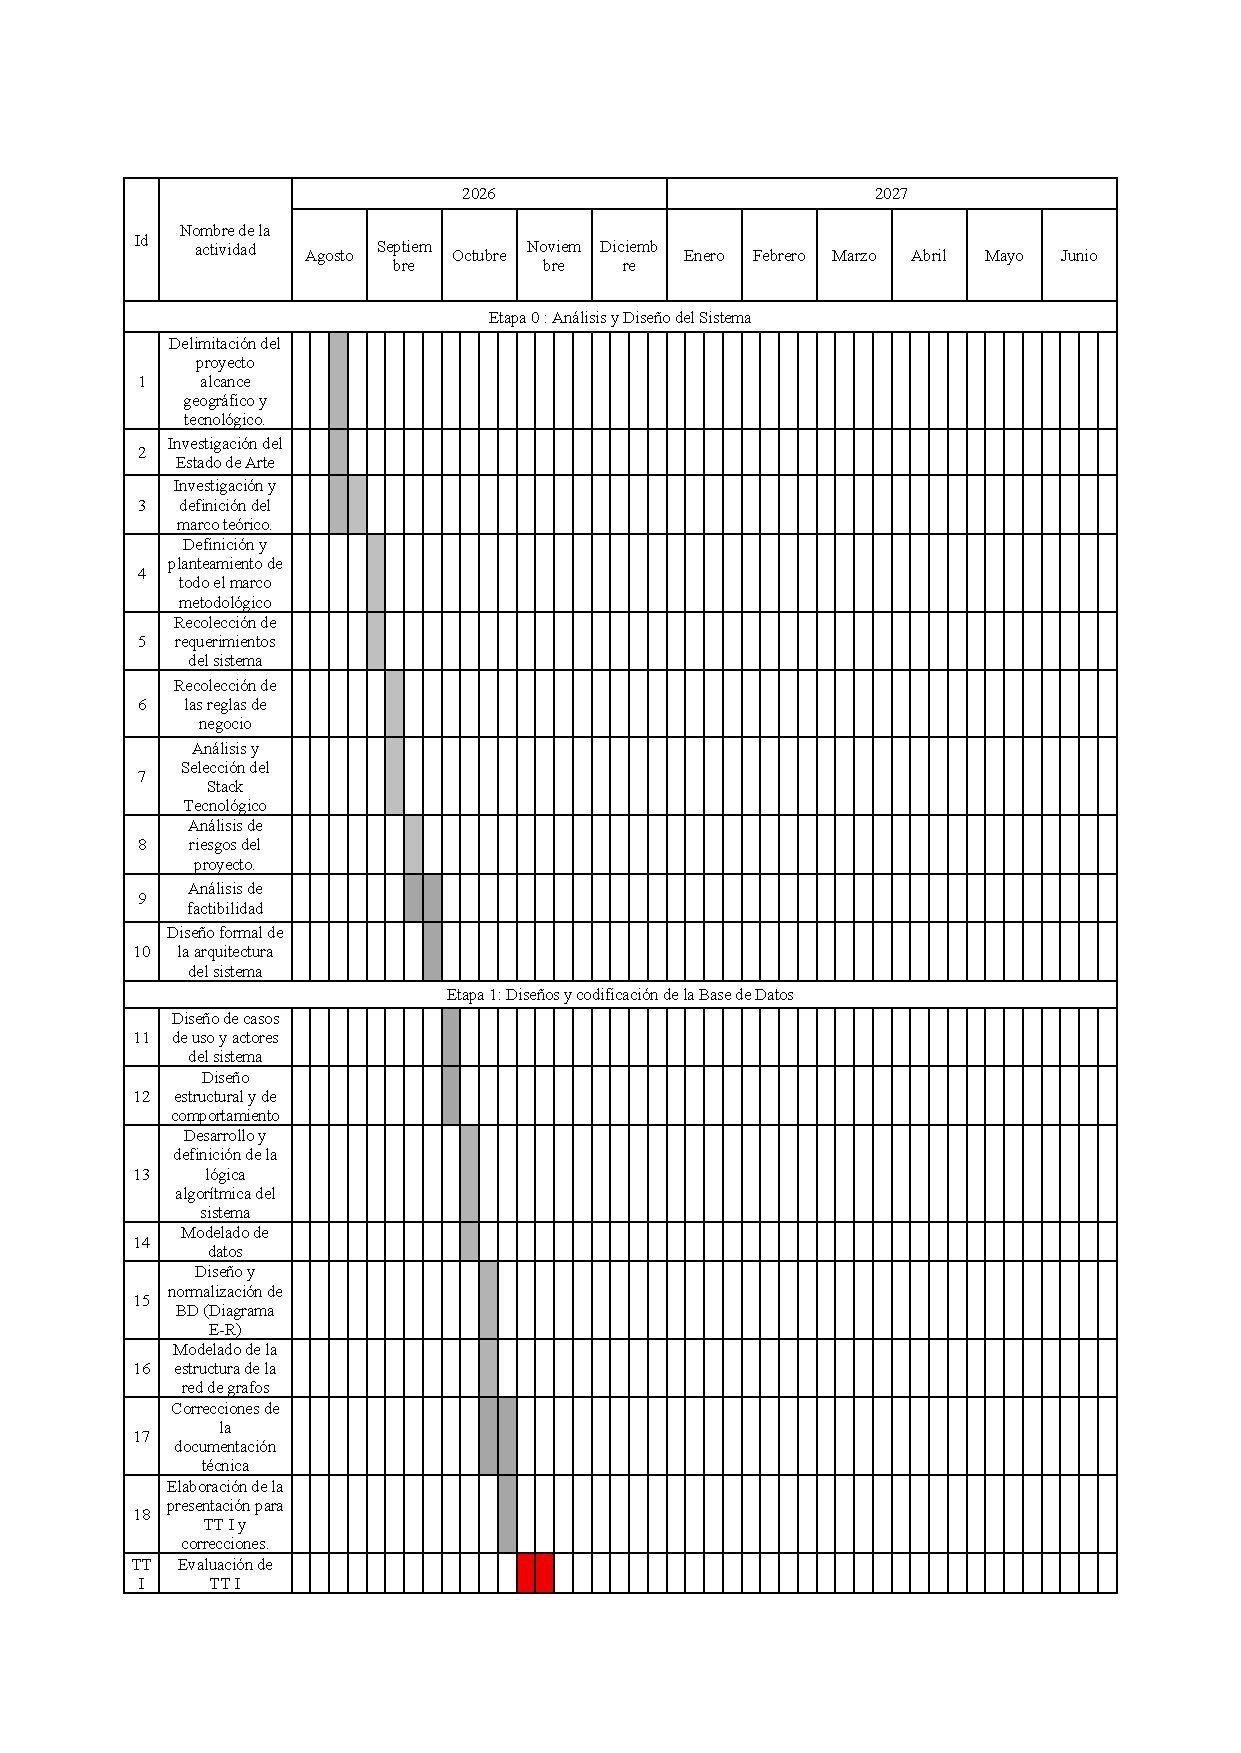
\includegraphics[width=\textwidth, trim={2cm 2cm 2cm 3cm}, clip]{figures/capitulo5_analisis_sistema/5.5_Analisis_de_Factibilidad/Cronograma_2027_TT1.pdf} 
    \caption{Diagrama de Gantt general de actividades del Trabajo Terminal}
    \label{fig:cronograma_actividades}
\end{figure}

\begin{figure}[H]
    \centering
    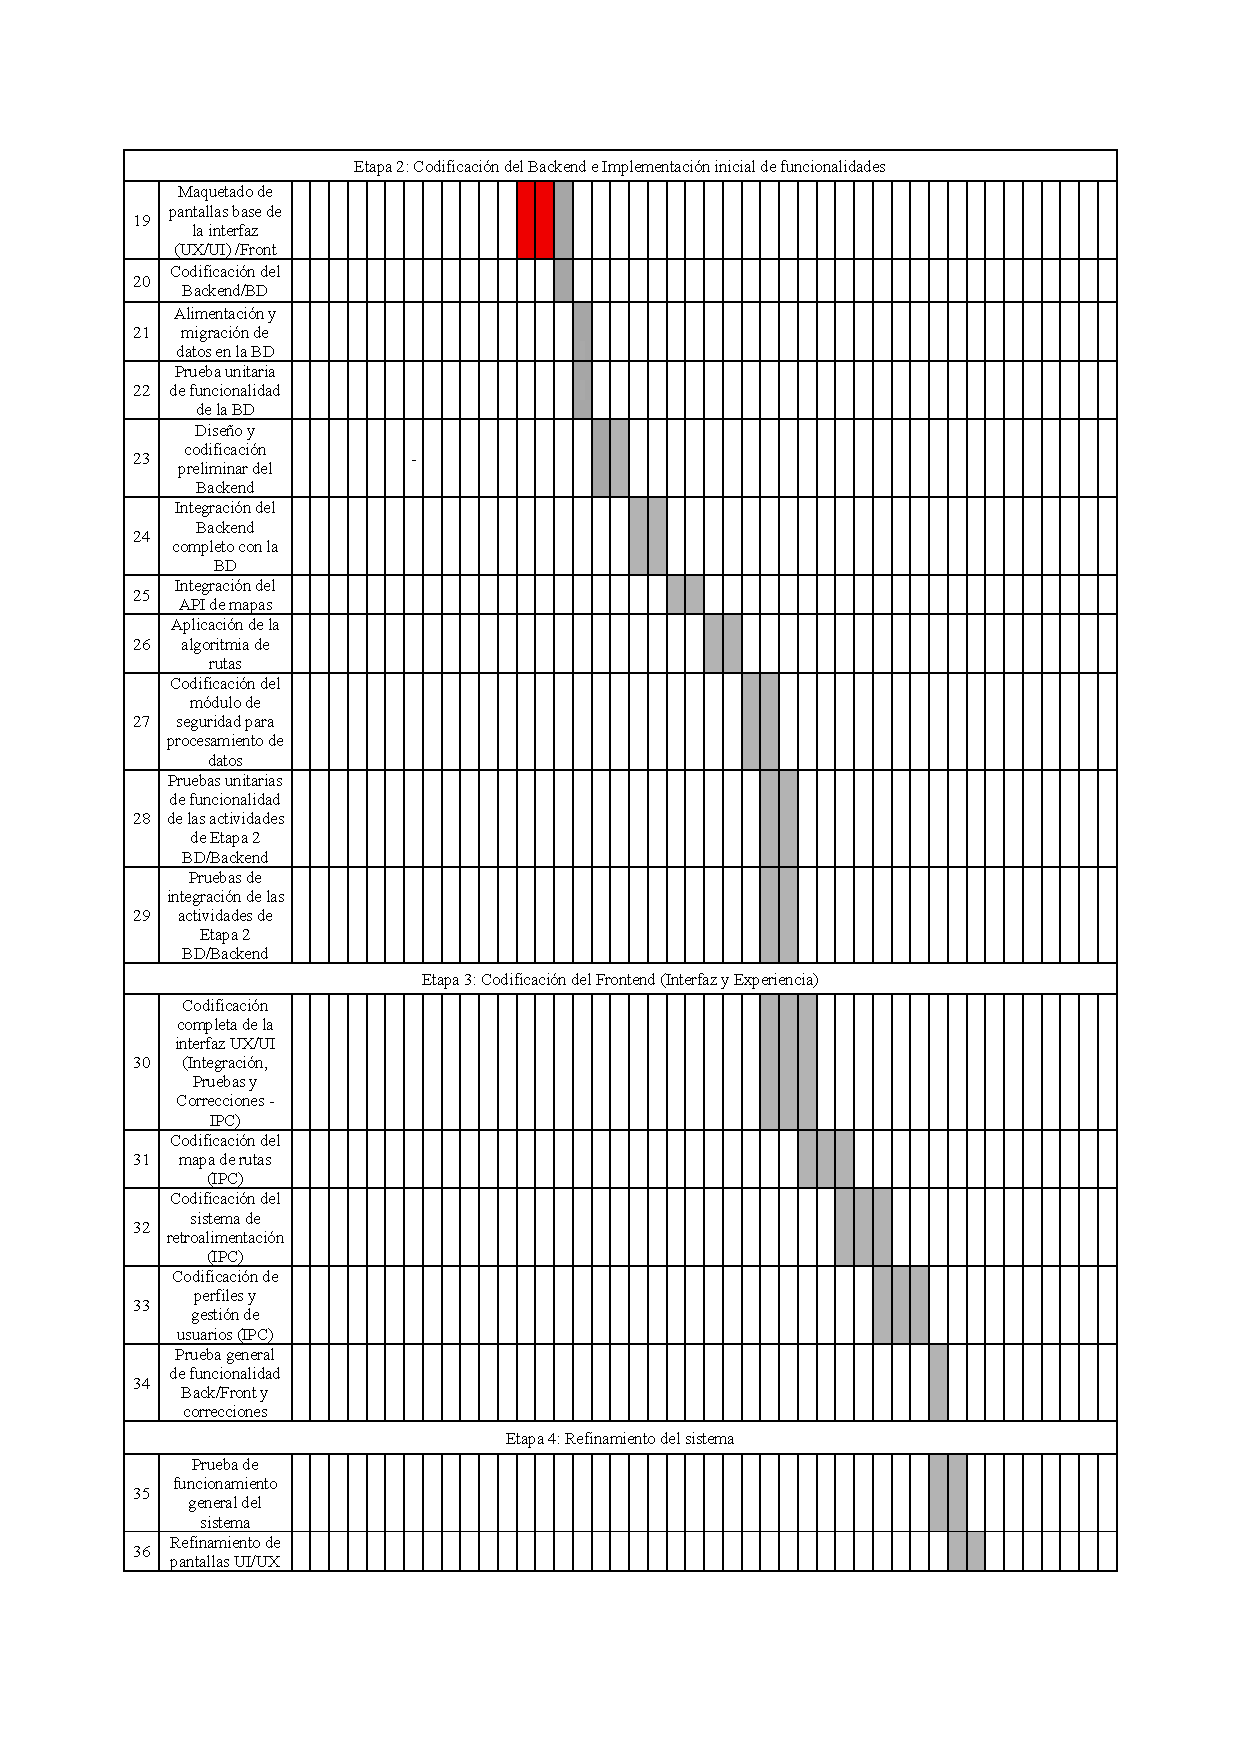
\includegraphics[width=\textwidth, trim={2cm 2cm 2cm 3cm}, clip]{figures/capitulo5_analisis_sistema/5.5_Analisis_de_Factibilidad/Cronograma_2027_TT1-1-2-2.pdf} 
    \caption*{Continuación del diagrama \ref{fig:cronograma_actividades}}
\end{figure}

\begin{figure}[H]
    \centering
    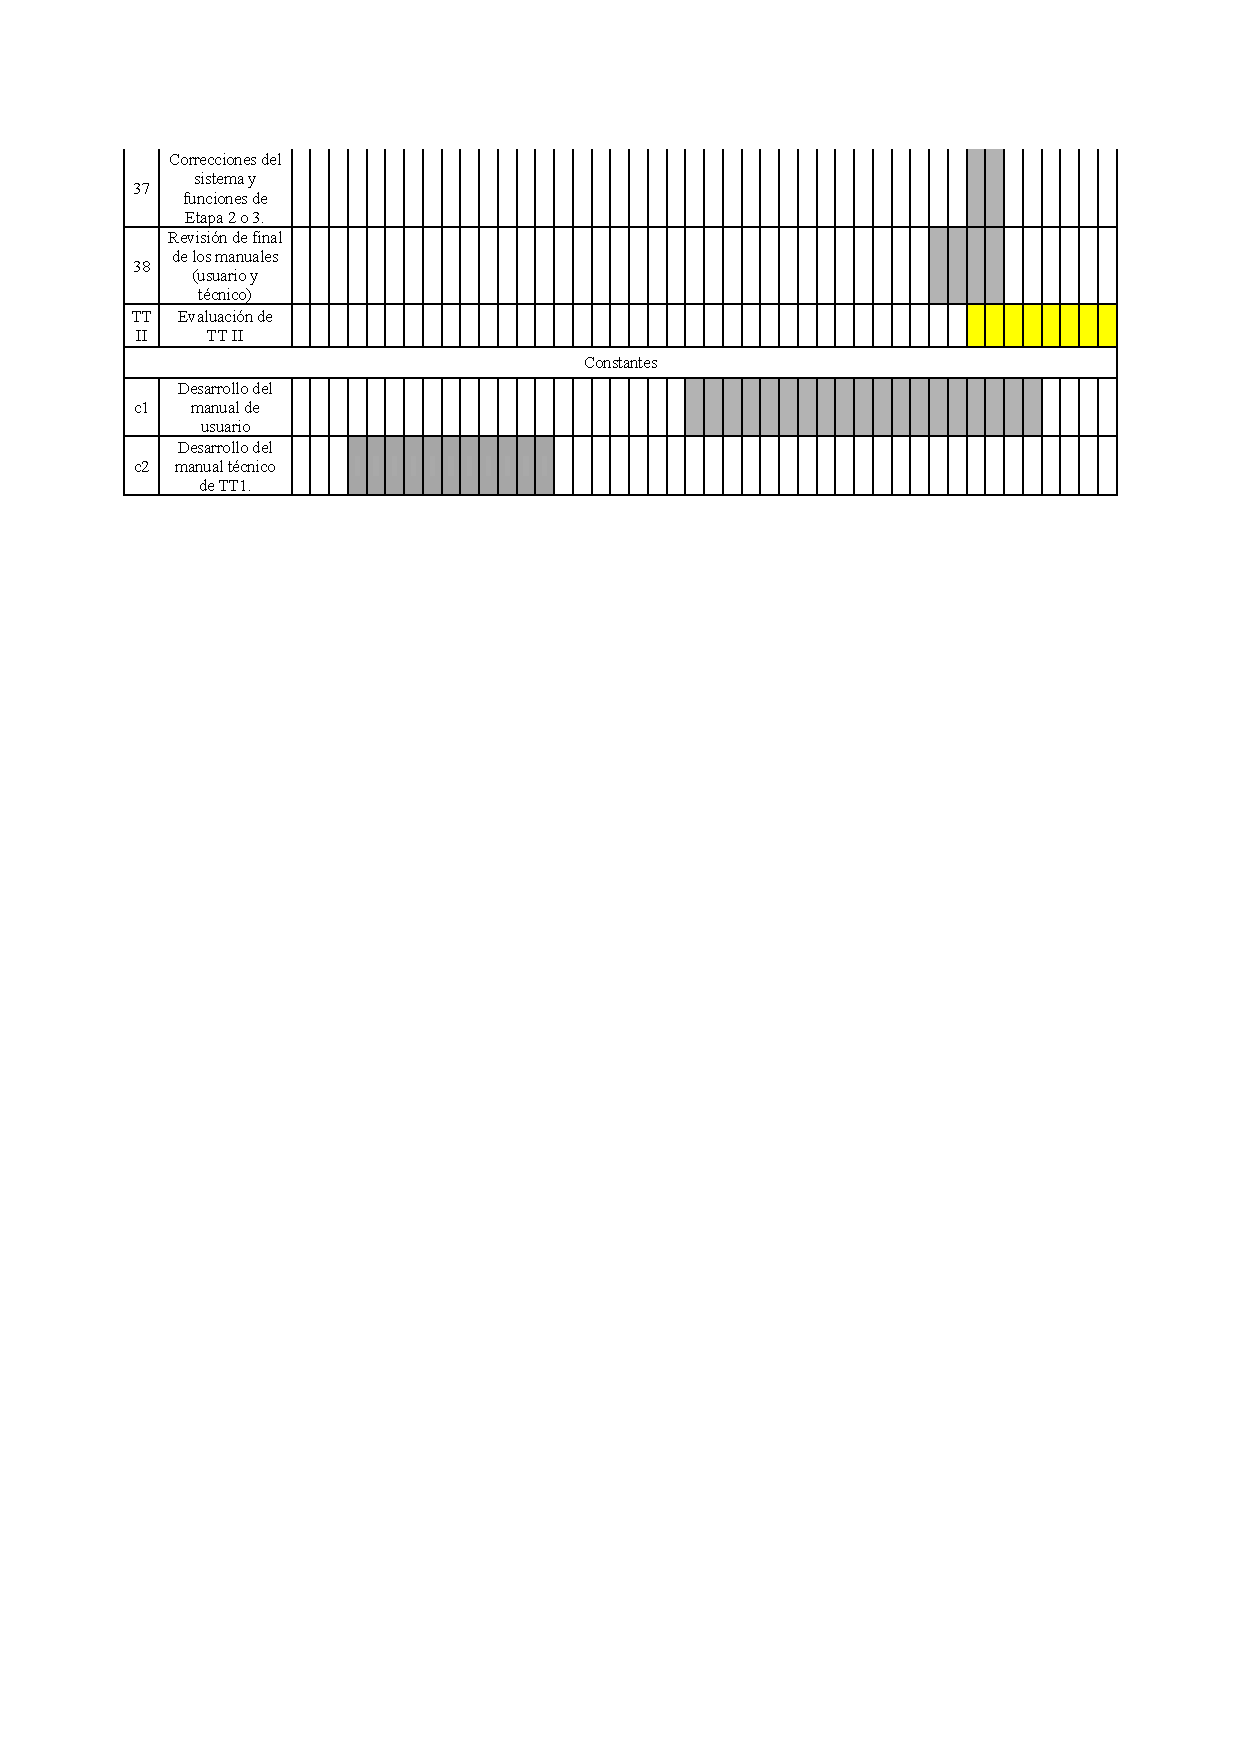
\includegraphics[width=\textwidth, trim={2cm 21cm 2cm 2cm}, clip]{figures/capitulo5_analisis_sistema/5.5_Analisis_de_Factibilidad/Cronograma_2027_TT1-3.pdf} 
    \caption*{Continuación del diagrama \ref{fig:cronograma_actividades}}
\end{figure}

Es necesario realizar la comparación entre el diagrama de Gantt (plazos definidos) contra el tiempo real requerido para el proyecto, de esta forma se observa si realmente el sistema es factible dentro de los intervalos de tiempo establecidos.

En la tabla \ref{tab:resumen_dias} se calcula el tiempo de esfuerzo requerido en base a la cantidad de horas de trabajo que el equipo invierte en el sistema obteniendo la cantidad de días laborales (tomando en cuenta una jornada de tiempo completo; 8 horas) necesarios para el desarrollo dentro del intervalo general de tiempo. 

El plazo de trabajo parte en la tercera semana de Agosto de 2026 y finaliza hasta mediados de Mayo del 2027, considerando que las fechas de presentación de TT I-II se realizan aproximadamente un mes antes de la finalización del periodo escolar. 

\begin{table}[H]
\centering
\renewcommand{\arraystretch}{1.2}
\resizebox{\textwidth}{!}{
\begin{tabular}{l c c c c c c c}
\hline
\textbf{Mes} & \textbf{Días} & \textbf{\makecell{Fin de\\semana}} & \textbf{\makecell{Días no\\laborales}} & \textbf{\makecell{Días\\hábiles}} & \textbf{\makecell{Horas de\\trabajo\\por día\\(promedio)}} & \textbf{\makecell{Horas\\totales}} & \textbf{\makecell{Días\\laborales\\(8 horas\\al día)}} \\ \hline
\textbf{Agosto} & 15 & 4 & 0 & 11 & 4 & 44 & 5.5 \\ 
\textbf{Septiembre} & 30 & 8 & 1 & 21 & 4 & 84 & 10.5 \\ 
\textbf{Octubre} & 31 & 9 & 0 & 22 & 4 & 88 & 11 \\ 
\textbf{Noviembre} & 30 & 9 & 2 & 19 & 4 & 76 & 9.5 \\ 
\textbf{Diciembre} & 30 & 8 & 0 & 22 & 4 & 88 & 11 \\ 
\textbf{Enero} & 31 & 10 & 1 & 20 & 4 & 80 & 10 \\ 
\textbf{Febrero} & 28 & 8 & 1 & 19 & 4 & 76 & 9.5 \\ 
\textbf{Marzo} & 31 & 8 & 3 & 20 & 4 & 80 & 10 \\ 
\textbf{Abril} & 30 & 8 & 5 & 17 & 4 & 68 & 8.5 \\ 
\textbf{Mayo} & 31 & 10 & 2 & 19 & 4 & 76 & 9.5 \\ 
\textbf{Junio} & 7 & 2 & 0 & 5 & 4 & 20 & 2.5 \\ \hline
\textbf{Total} & \textbf{294} & \textbf{84} & \textbf{15} & \textbf{195} & & \textbf{780} & \textbf{97.5} \\ \hline
\end{tabular}
} 
\caption{Resumen de días para el desarrollo del proyecto (Agosto 2026 - Junio 2027) con base a los plazos establecidos en el Diagrama de Gantt \ref{fig:cronograma_actividades}.}
\label{tab:resumen_dias}
\end{table}

Como se aprecia en la tabla \ref{tab:resumen_dias} se cuentan con aproximadamente 98 días laborales para el desarrollo del trabajo terminal considerando una jornada laboral de 8 días, eliminando días festivos, fines de semana y periodos que no entran en el intervalo de tiempo.

%Pendiente por desarrollar el calculo del tiempo real con formulas matematicas de cada actividad para la estimacion real de esfuerzo en tiempo requerido y el contraste con los plazos ya definidos.                                                                                                                                                                                                                            




\subsection{Factibilidad económica}
\label{sec:factibilidad_economica}
A continuación se presenta el análisis de costos asociados al desarrollo del prototipo de aplicación móvil. Los costos de recursos humanos se calculan con base en tarifas de mercado vigentes para cada rol, con el fin de dimensionar el valor económico del trabajo invertido. Por otra parte, los recursos tecnológicos sí representan egresos reales derivados del uso de servicios externos necesarios para el preprocesamiento de datos del sistema. Todos los costos se expresan en pesos mexicanos (MXN) y se acompañan de la fuente y fecha de consulta correspondiente.

\paragraph{Recursos humanos}

Para la realización del proyecto se contempla la participación del equipo de trabajo terminal, compuesto por tres integrantes que colaboran de manera conjunta en todas las etapas del desarrollo, especializándose respectivamente en el diseño y construcción de la base de datos y la lógica algorítmica, el desarrollo de la aplicación móvil, y el análisis y tratamiento de los datos geoespaciales y delictivos. Dado que el proyecto se desarrolla bajo la metodología Scrumban, las funciones de coordinación del equipo son rotativas entre sus integrantes y se ejercen dentro del mismo horario de trabajo individual, por lo que no representan un costo adicional de recursos humanos.

Se considera una dedicación de 2 horas diarias por integrante a lo largo del periodo efectivo de desarrollo del proyecto, comprendido entre el 24 de agosto de 2026 y mediados de mayo de 2027 (aproximadamente 9 meses) conforme al cronograma de actividades. De acuerdo con el Calendario Escolar 2026-2027 del Instituto Politécnico Nacional \cite{ipn_calendario2026}, el cálculo de días hábiles efectivos se obtiene de la siguiente manera:

\begin{align*}
\text{Días hábiles totales (24 ago. 2026 -- 15 may. 2027)} &= 190 \\
(-)\ \text{Días festivos (descanso obligatorio y acuerdo sindical)} &= 12 \\
(-)\ \text{Periodos vacacionales (dic.--ene. y mar.--abr.)} &= 22 \\
\hline
\text{Días hábiles efectivos} &= 156
\end{align*}

\[
156 \text{ días} \times 2 \text{ horas/día} = 312 \text{ horas efectivas por integrante}
\]

La Tabla~\ref{tab:sueldos_mercado} presenta el sueldo mensual promedio en México para cada rol del equipo, obtenido de fuentes de empleo consultado el 6 de octubre del 2026.

\begin{table}[H]
    \centering
    \caption[Sueldo mensual promedio por rol]{Sueldo mensual promedio por rol, según datos de mercado.}
    \vspace{0.2cm}
    \resizebox{\textwidth}{!}{%
    \begin{tabular}{|l|l|c|}
        \hline
        \textbf{Cargo} & \textbf{Fuente} & \textbf{Sueldo mensual promedio} \\ \hline
        Backend Developer & Indeed México \cite{indeed_backend_developer} & \$ 19,210.00 \\ \hline
        Analista de Datos & Indeed México \cite{indeed_analistas_datos} & \$ 15,221.00 \\ \hline
        Desarrollador Móvil & Indeed México \cite{indeed_android_developer} & \$ 17,302.00 \\ \hline
    \end{tabular}%
    }
    \label{tab:sueldos_mercado}
\end{table}

El costo por hora de cada rol se obtiene dividiendo el sueldo mensual promedio entre 160 horas mensuales, correspondientes a una jornada estándar de 8 horas diarias durante 20 días hábiles al mes. Este costo por hora se multiplica por las 312 horas efectivas estimadas por integrante, obteniendo el costo total de recursos humanos mostrado en la Tabla~\ref{tab:recursos_humanos}.

\begin{table}[H]
    \centering
    \caption[Recursos humanos necesarios para realizar el proyecto]{Recursos humanos necesarios para realizar el proyecto. Elaboración propia.}
    \vspace{0.2cm}
    \resizebox{\textwidth}{!}{%
    \begin{tabular}{|l|c|c|c|}
        \hline
        \textbf{Cargo} & \textbf{Horas estimadas} & \textbf{Costo/hora} & \textbf{Costo total} \\ \hline
        Backend Developer & 312 & \$ 120.06 & \$ 37,458.72 \\ \hline
        Analista de Datos & 312 & \$ 95.13 & \$ 29,680.56 \\ \hline
        Desarrollador Móvil & 312 & \$ 108.14 & \$ 33,739.68 \\ \hline
        \multicolumn{3}{|r|}{\textbf{Total}} & \textbf{\$ 100,878.96} \\ \hline
    \end{tabular}%
    }
    \label{tab:recursos_humanos}
\end{table}


\paragraph{Recursos tecnológicos}

Para la realización del proyecto se contempla el uso de los siguientes recursos de hardware, software y servicios en la nube. El equipo de cómputo empleado es propiedad de los integrantes del equipo, por lo que no representa un costo de adquisición adicional para el proyecto. El consumo eléctrico y de internet asociado a su uso durante el desarrollo se contabiliza por separado en la sección de Recursos materiales. Para el desarrollo de la aplicación móvil se emplea el framework Flutter (Dart), mientras que para la gestión de la base de datos y el motor de ruteo geoespacial se utiliza Supabase (PostgreSQL con las extensiones PostGIS y pgRouting), justificado técnicamente en la sección~\ref{sec:factibilidad_técnica}.

El plan gratuito de Supabase ofrece 500 MB de base de datos, 500 MB de almacenamiento de archivos, 5 GB de transferencia de datos mensual y solicitudes de API ilimitadas \cite{supabase_pricing}. El polígono de estudio delimitado en la Figura~\ref{fig:mapa_zona_estudio} abarca una superficie de 26.31 km\textsuperscript{2} y su red vial comprende aproximadamente 11{,}700 segmentos de calle. Considerando un peso promedio de 1 a 3 KB por segmento, el volumen estimado de la base de datos se ubica entre 12 y 35 MB, muy por debajo del límite mencionado, por lo que se opta por el plan gratuito.

Para el preprocesamiento de la información se emplea la Street View Static API de Google Maps Platform, mediante la cual se obtendrán tres imágenes por cada segmento de calle, es decir, aproximadamente 35{,}100 solicitudes. Esta API ofrece una cuota gratuita de 10{,}000 solicitudes mensuales y cobra \$7.00 USD por cada 1{,}000 solicitudes adicionales \cite{google_maps_pricing}, por lo que se generarían 25{,}100 solicitudes facturables, equivalentes a \$175.70 USD (\$3,156.80 MXN). Posteriormente, las imágenes se analizan con el modelo Qwen3.7-Flash \cite{qwen_pricing}, cuyo costo para solicitudes de hasta 32{,}000 tokens es de \$0.03 USD por millón de tokens de entrada y \$0.13 USD por millón de tokens de salida. Considerando un consumo aproximado de 2{,}000 tokens de entrada y 500 de salida por imagen, el análisis de las 35{,}100 imágenes requiere 70.2 millones de tokens de entrada y 17.55 millones de salida, con un costo total de \$4.39 USD (\$78.83 MXN). Durante la operación de la aplicación se utiliza el SDK de Maps para dispositivos móviles, cuyo uso es ilimitado y sin costo, y Places API (New), cuyas SKU de Autocomplete y Place Details Essentials incluyen 10{,}000 solicitudes gratuitas mensuales cada una \cite{google_maps_pricing}. Los montos expresados en dólares estadounidenses se convirtieron a pesos mexicanos con el tipo de cambio FIX publicado por el Banco de México el 6 de octubre de 2026, equivalente a \$17.9670 MXN por dólar \cite{banxico_fix}.

Adicionalmente, el equipo utiliza dos servicios por suscripción mensual durante el desarrollo del proyecto: Overleaf, para la redacción del documento en LATEX, y Udemy, para la capacitación técnica de los integrantes. Considerando una duración de nueve meses, el costo de estos servicios se desglosa en la Tabla~\ref{tab:servicios_adicionales}.

El proyecto contempla como entregable un prototipo funcional de la aplicación móvil, cuya conclusión no depende de su publicación en una tienda de aplicaciones. No obstante, de presentarse la oportunidad, el prototipo podrá publicarse en Google Play Store, lo que requiere un pago único de registro de desarrollador de \$25.00 USD (\$449.18 MXN) \cite{google_play_console}. Al tratarse de un gasto opcional, no se incluye en el total del presupuesto.

\begin{table}[H]
    \centering
    \caption[Recursos tecnológicos necesarios para realizar el proyecto]{Recursos tecnológicos necesarios para realizar el proyecto. Elaboración propia.}
    \vspace{0.2cm}
    \resizebox{\textwidth}{!}{%
    \begin{tabular}{|l|l|c|}
        \hline
        \textbf{Cantidad} & \textbf{Descripción} & \textbf{Costo} \\ \hline
        \multicolumn{3}{|l|}{\textit{Hardware}} \\ \hline
        3 & Equipo de cómputo propio del equipo & \$ 0.00 \\ \hline
        \multicolumn{3}{|l|}{\textit{Software y servicios en la nube}} \\ \hline
        1 & Flutter / Dart (código abierto) & \$ 0.00 \\ \hline
        1 & Supabase -- plan gratuito (PostgreSQL, PostGIS, pgRouting) & \$ 0.00 \\ \hline
        1 & Git / GitHub (plan gratuito) & \$ 0.00 \\ \hline
        1 & Google Meet (plan gratuito) & \$ 0.00 \\ \hline
        1 & Notion (plan estudiante, gratuito) & \$ 0.00 \\ \hline
        \multicolumn{3}{|l|}{\textit{APIs de preprocesamiento (35{,}100 imágenes: 11{,}700 segmentos $\times$ 3)}} \\ \hline
        35{,}100 & Google Street View Static API (10{,}000 gratuitas; 25{,}100 a \$7.00 USD/1{,}000) & \$ 3,156.80 \\ \hline
        35{,}100 & Qwen3.7-Flash, análisis de imágenes (70.2 M tokens de entrada y 17.55 M de salida) & \$ 78.83 \\ \hline
        \multicolumn{3}{|l|}{\textit{APIs de operación de la aplicación}} \\ \hline
        1 & Maps SDK para móvil (uso ilimitado sin costo) & \$ 0.00 \\ \hline
        1 & Places API (New), dentro de la cuota gratuita & \$ 0.00 \\ \hline
        \multicolumn{3}{|l|}{\textit{Opcional (no incluido en el total)}} \\ \hline
        1 & Registro de desarrollador Google Play (pago único) & \$ 449.18 \\ \hline
        \multicolumn{2}{|r|}{\textbf{Total}} & \textbf{\$ 3,235.63} \\ \hline
    \end{tabular}%
    }
    \label{tab:recursos_tecnologicos}
\end{table}

\begin{table}[H]
    \centering
    \caption[Servicios adicionales por suscripción mensual]{Servicios adicionales por suscripción mensual. Elaboración propia.}
    \vspace{0.2cm}
    \resizebox{\textwidth}{!}{%
    \begin{tabular}{|c|l|c|c|}
        \hline
        \textbf{Meses} & \textbf{Descripción} & \textbf{Costo mensual} & \textbf{Costo total} \\ \hline
        9 & Overleaf (suscripción mensual) & \$ 99.00 & \$ 891.00 \\ \hline
        9 & Udemy (suscripción mensual) & \$ 209.00 & \$ 1,881.00 \\ \hline
        \multicolumn{3}{|r|}{\textbf{Total}} & \textbf{\$ 2,772.00} \\ \hline
    \end{tabular}%
    }
    \label{tab:servicios_adicionales}
\end{table}

\paragraph{Recursos materiales}

Para la realización del proyecto se contemplan los siguientes recursos materiales asociados a la operación básica del equipo de trabajo. El costo de la energía eléctrica se estima a partir del consumo de los equipos de cómputo durante las horas efectivas de trabajo. Considerando las 312 horas efectivas por integrante calculadas en la sección de recursos humanos, y una potencia aproximada de 65 W por equipo, el consumo se obtiene de la siguiente manera:

\begin{align*}
\text{Horas de uso} &= 312 \text{ h} \times 3 \text{ integrantes} = 936 \text{ h} \\
\text{Consumo} &= 936 \text{ h} \times 0.065 \text{ kW} = 60.84 \text{ kWh} \approx 61 \text{ kWh}
\end{align*}

Dicho consumo se valora con la cuota del consumo excedente de la Tarifa 1 de la Comisión Federal de Electricidad para octubre de 2026, equivalente a \$4.054 por kilowatt-hora \cite{cfe_tarifa1}, considerada como valor conservador. Respecto al servicio de internet, cada integrante cuenta con un paquete residencial de 100 Mbps con costo mensual de \$390.00 \cite{totalplay_paquetes}, el cual se contabiliza durante los 9 meses de desarrollo del proyecto.

\begin{table}[H]
    \centering
    \caption[Recursos materiales necesarios para realizar el proyecto]{Recursos materiales necesarios para realizar el proyecto. Elaboración propia.}
    \vspace{0.2cm}
    \resizebox{\textwidth}{!}{%
    \begin{tabular}{|l|l|c|c|}
        \hline
        \textbf{Cantidad} & \textbf{Descripción} & \textbf{Costo} & \textbf{Total} \\ \hline
        61 & Energía eléctrica, Tarifa 1 CFE (kWh) & \$ 4.054 & \$ 247.29 \\ \hline
        27 & Internet residencial 100 Mbps (3 integrantes $\times$ 9 meses) & \$ 390.00 & \$ 10,530.00 \\ \hline
        \multicolumn{3}{|r|}{\textbf{Total}} & \textbf{\$ 10,777.29} \\ \hline
    \end{tabular}%
    }
    \label{tab:recursos_materiales}
\end{table}


\paragraph{Flujo de pago}

El costo total estimado del proyecto se resume en la Tabla~\ref{tab:flujo_pago} y asciende a \$129,430.27 MXN, que resulta de sumar los recursos humanos, tecnológicos y materiales (\$117,663.88 MXN) y un 10\% de imprevistos calculado sobre dicho subtotal (\$11,766.39 MXN). No se considera el pago opcional de registro en Google Play Store. De este monto, \$100,878.96 corresponden al valor de mercado del trabajo del equipo, el cual, al ser realizado directamente por los integrantes del trabajo terminal sin una relación de contratación formal, no representa un desembolso. De igual forma, los recursos materiales (energía eléctrica e internet) corresponden a servicios que los integrantes ya tienen contratados, por lo que se contabilizan para dimensionar el costo real del proyecto sin implicar un gasto adicional. En consecuencia, el egreso efectivo se limita a los recursos tecnológicos, por un monto de \$6,007.63 MXN, equivalente a aproximadamente \$2,002.54 MXN por integrante a lo largo de los nueve meses de desarrollo (\$222.50 MXN mensuales).

Con base en lo anterior, el proyecto se considera económicamente viable: el gasto efectivo es reducido y proviene principalmente de servicios de preprocesamiento de uso único y de suscripciones mensuales, mientras que el resto de los costos corresponde a trabajo y recursos que el equipo ya posee o tiene contratados.

\begin{table}[H]
    \centering
    \caption[Resumen de costos totales del proyecto]{Resumen de costos totales del proyecto. Elaboración propia.}
    \vspace{0.2cm}
    \begin{tabular}{|l|c|}
        \hline
        \textbf{Recursos} & \textbf{Costo} \\ \hline
        Recursos Humanos & \$ 100,878.96 \\ \hline
        Recursos Tecnológicos & \$ 6,007.63 \\ \hline
        Recursos Materiales & \$ 10,777.29 \\ \hline
        Subtotal & \$ 117,663.88 \\ \hline
        Imprevistos (10\%) & \$ 11,766.39 \\ \hline
        \textbf{Total} & \textbf{\$ 129,430.27} \\ \hline
    \end{tabular}
    \label{tab:flujo_pago}
\end{table}

\subsection{Factibilidad legal}
\label{sec:factibilidad_legal}
En este apartado se analiza la factibilidad legal del proyecto, donde se verifica el cumplimiento de los requisitos jurídicos y si esta dentro de las leyes, normas y reglamentos vigentes del marco jurídico sin llegar a infringir leyes, derechos de autor o licencias de terceros.  



\subsection{Factibilidad de recursos}
\label{sec:factibilidad_recursos}
\input{documents/capitulo5_analisis_sistema/5.5_Analisis_de_Factibilidad/5.5.5_Factibilidad_recursos/seccion5_5_5}



